% Copyright (c)) 2014,2016 Casper Ti. Vecto  
% Public domain 
\chapter{系统需求分析}

透过特性要因分析可以将比特币的交易监督系统大致分为四个主题,如图\ref{fish1}所示,分别为信息安全技术、加密货币钱包、近场通信技术以及数据库。作为⼀个⾦流系统,四项主轴之中信息安全是不可或缺的环节,着重于商家认证机制、用户权限控管、身份识别管理、用户访问控制四个方向;本系统致力于奠定匿名对实名的加密货币系统,必须对区块链技术、公钥私钥生成算法、点对点交易技术、钱包地址产出以及货币发行技术五个方向进行探讨;在交易场景中,本系统采用近场通信技术,因此需要对商品RFID标签建置、读取商品RFID标签以及Android Beam传输商品交易进行基础的API调研;为了使加密货币实名制的实现,数据库必须存储与政府和商家相关的信息。此时数据库加密、个人信息去识别化安全以及数据库连接便相当重要。
		\begin{figure}[!htb]
			\centering
			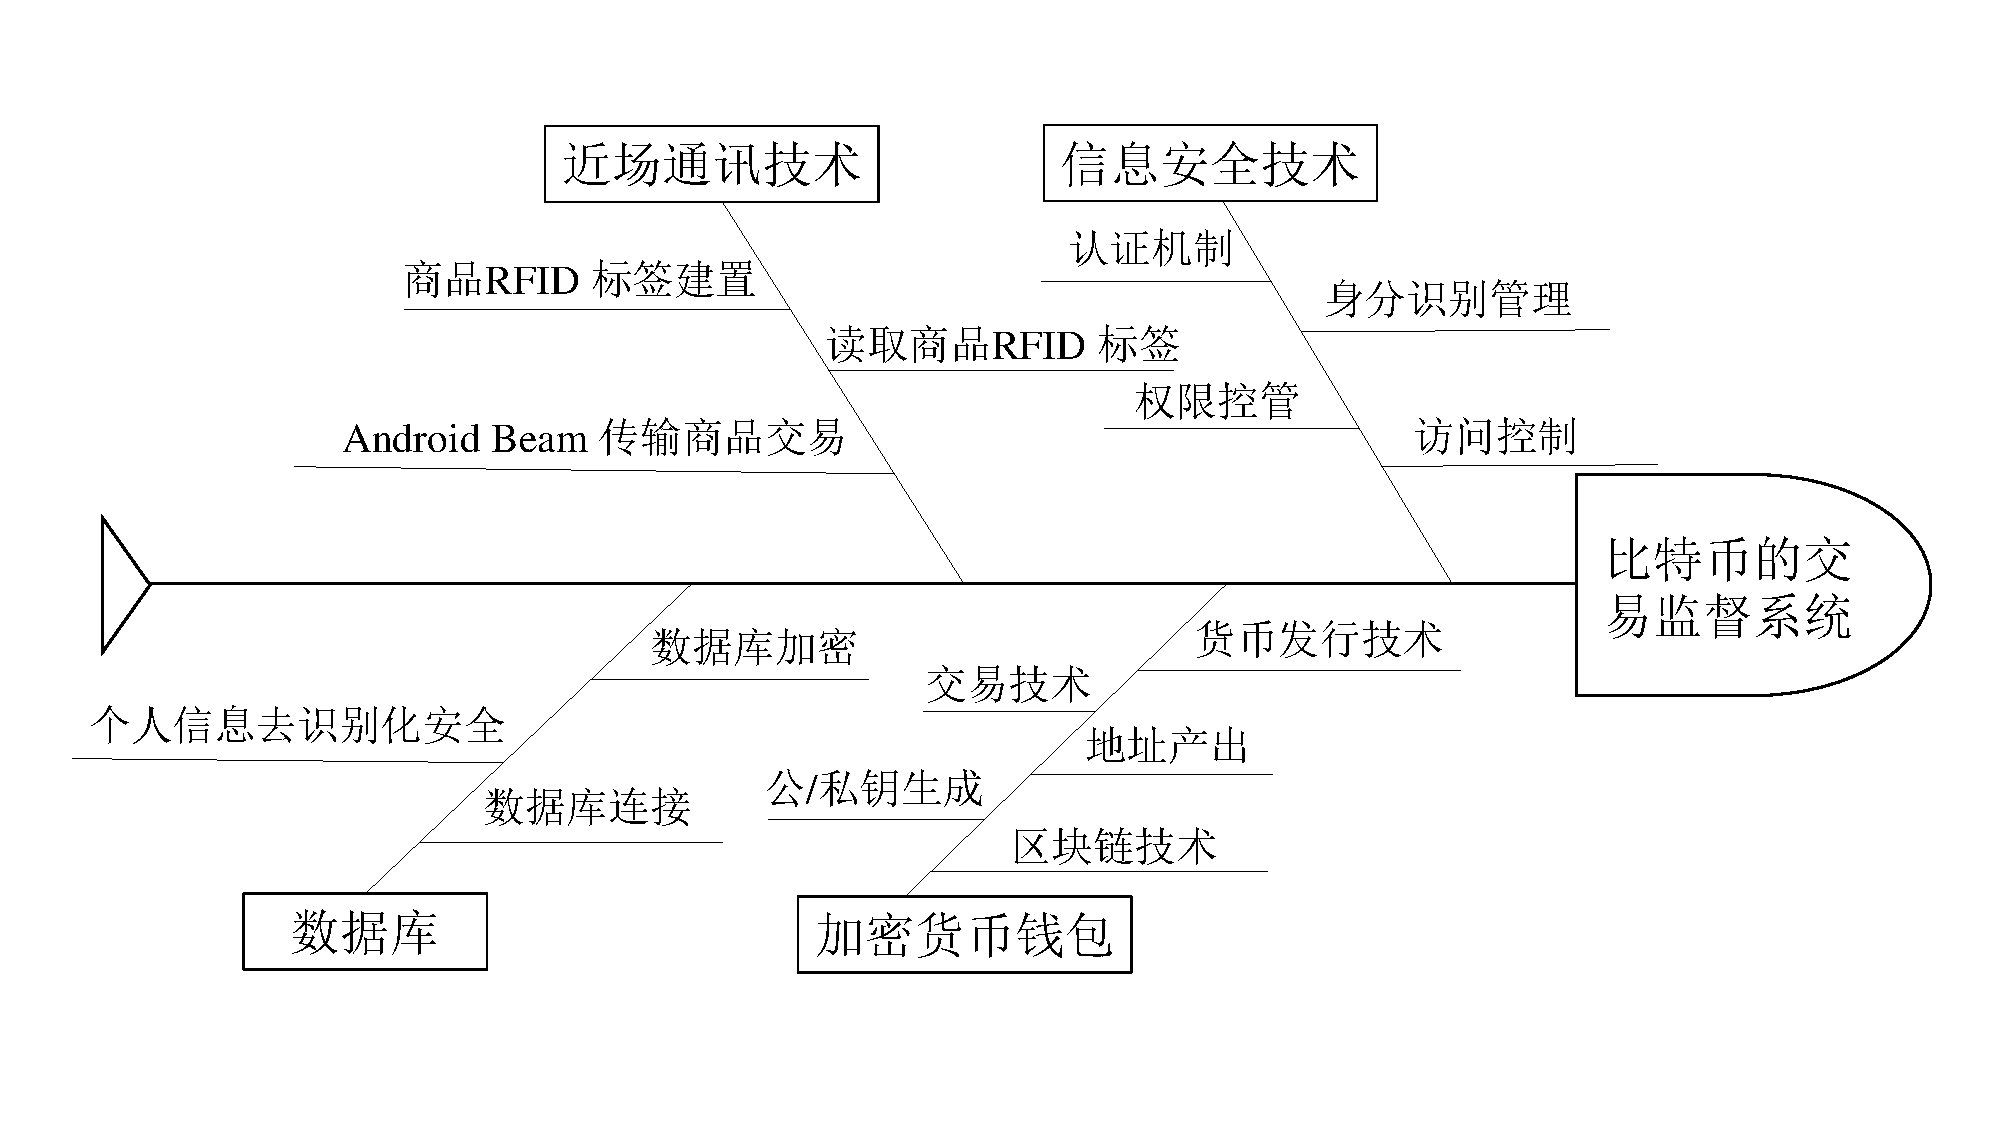
\includegraphics[width = 0.8\textwidth]{fish1.pdf}
			\caption{⽐特币的交易监督系统特性要因分析图}\label{fish1}
		\end{figure}

为了使本⽂所提出的系统设计之模块更加明确,对系统进⾏详细的需求分析可以使应确⽴的⽅向更加分明,在本章将分为三节进行分析,分别为交易模型分析、功能性需求分析以及非功能性需求分析。


\section{交易模型分析}

在设计比特币的交易监督系统之前必须针对现今社会中人与人之间的交易方式进行分析,在支付的方式依照使用人数比例大致可区分为现金交易以及电子支付两种类别,图\ref{modeall}为各种交易模型示意图。
%%fig allan
\begin{figure}[!htb]
	\centering
	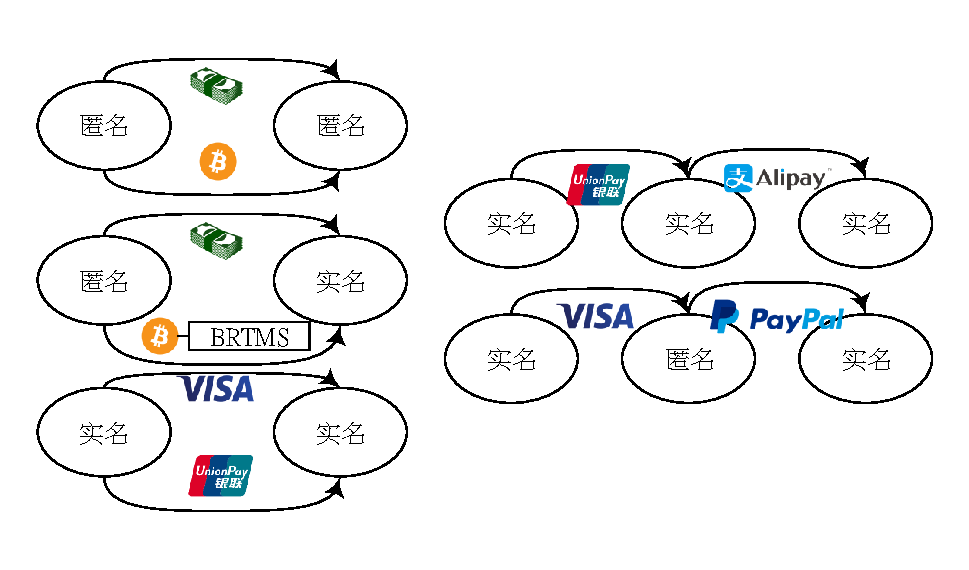
\includegraphics[width = 0.7\textwidth]{modeall.pdf}
	\caption{各种交易模型示意图}\label{modeall}
\end{figure}

	\subsection{现金交易类型}
	在现金交易模型中大致分为匿名顾客支付匿名商家以及匿名顾客支付实名商家两种,在过去的社会中,贝壳货币逐渐的被黄金取代,但黄金过于沈重在交易上相当不便。纸钞渐渐取代⿈⾦,法定货币的概念因此形成。法定货币包括钞票以及钱币,在过往的法定货币存在着黄金价值支撑,使得法定货币具有价值,但经过历史的变迁,已无⼤量的黄金作为法定货币的价值⽀撑,使法定货币渐渐地⾛向信⽤本位,纸钞以及铜币的使用皆不带有持有者的真实姓名,因此在现金交易模型分析中将顾客支付皆归类为匿名支付。

		\subsubsection{(一)匿名顾客支付匿名商家交易模型}
		现金法定货币的本身不存在用户信息以及交易信息。现⾦是一种匿名的支付方式,早期有许多的商家并无向政府进行注册,当顾客完成挑选商品进行结帐的同时,顾客只是将现金货币交付给商家,商家将商品卖给顾客,但在这过程中并无开立交易凭据。在商家无开立交易凭据的情况下,顾客完成此次的交易后,倘若该商品存在着瑕疵,进而引起商家与顾客之间的消费纠纷,使其在追溯的过程中存在没有凭据的困扰。对于匿名顾客支付匿名商家可以保有顾客的信息隐私,但无法保障顾客应有的顾客权益。政府因没有交易凭据而无法确认消费行为存在,使政府在课征税收的过程变得困难,且商家所贩售的商品并无得到明确的信息纪录,对于商家库存管理只能依靠过去的经验。对政府而言,商家贩售的商品并无完整的商品信息,无法对商家商品进行安全性检验,使得国民购买的商品存在的许多安全疑虑。

		\subsubsection{(二)匿名顾客支付实名商家交易模型}
		现⾦最为常⾒的為匿名顾客⽀付给实名商家的交易模式,在匿名顾客以现⾦法定货币进⾏交易时,商家只要开⽴交易凭据,即被归类为匿名顾客⽀付实名商家交易模型。商家在开⽴交易凭据的同时,凭据上所记载的信息包括职⼯信息、商家信息以及产品信息;职⼯信息记录该笔交易的担当人员,商家信息记录商家与顾客创建交易行为的时间与地点,产品信息详细记录顾客于该商家购买的商品;交易凭据因此成为记录交易事实的重要证明。对于顾客,因现⾦法定货币的匿名性使顾客依旧保有顾客信息隐私,但却因为商家开⽴交易凭据得以保障顾客权益。商家因为开⽴交易凭据使商家为实名,因为实名使得商家可以经营品牌形象。除此之外,因为凭据记录了产品信息让商家在库存管理以及收支计算变得更加容易。对政府⽽⾔,可以查看商家的所得以及商家贩售的商品,使政府可以更有效率的课征税收以及管理产品安全。

	\subsection{电子支付类型}
	电子商务的日趋盛⾏,电⼦支付交易模式也日渐普及,电子支付与加密货币的区块链技术不同的是采用数据库存储着所有的交易信息,而用户要能够使用电子支付也必须接受电子支付运营商实名制的条件。在电子支付的数据库中存在着黑客攻击、信息不一致以及中心化运营的风险,但电⼦⽀付有效解决了难以现金支付远距离之困境,也使得现今的网络购物变得更加发达。在电子支付交易模型中分为三种交易分别为实名顾客支付实名商家、实名顾客透过实名第三方再实名商家以及实名顾客透过匿名第三方再实名商家,以下将逐一说明。

		\subsubsection{(一)实名顾客支付实名商家交易模型}
		典型的实名顾客支付实名商家交易模式以VISA 国际电⼦⽀付公司为例,VISA 国际电⼦⽀付公司(以下简称为VISA 公司)为中⼼化的运营,⽤⼾在使用VISA 电⼦⽀付(以下简称为VISA 服务)前,必须做详尽的⽤户真实⾝份认证,这使得VISA公司可以得到⽤⼾的所有信息,因此VISA公司拥有了允许或冻结相关⽤⼾⼾头的使用权限,并且为了保护用户隐私,所有的交易信息记录皆被存储在VISA 公司的数据库当中。

		VISA公司透过不断的优化电⼦⽀付技术已经可以接受每秒两千笔的交易量,为了维持稳定的运营服务,VISA 公司对每笔交易收取固定⽐例的⼿续费。在使用VISA 服务的过程中,顾客因为必须进⾏实名验证,使得顾客必须透露顾客个⼈信息,甚⾄可以针对这些个⼈信息进⾏商业上的交易。商家必须承担VISA 服务所需的交易⼿续费,成本因此提高,使得商品售价必须做出相对应的调整。对政府⽽⾔,因为交易信息皆以中⼼化的⽅式存储,可以⽅便的查看,也可以快速的查阅商家收⼊课征应缴的税收。
		

		\subsubsection{(二)实名顾客透过实名第三方支付实名商家交易模型}
		电⼦⽀付⽅式⽇趋普及也使用户可选择的电⼦⽀付渠道更加多元,较为常⾒的包括VISA 电⼦⽀付以及银联电⼦⽀付,⽽每⼀家银⾏为了让用户能在电⼦商务的⽀付上更为便利,会同时推广电⼦⽀付,使得银⾏卡⽀持电⼦⽀付,但更多的银⾏卡林⽴使得用户在卡⽚管理上更加繁琐,第三⽅的支付集成平台开始出现成为解决⽅案。顾客可以先在实名第三⽅⽀付后台添加多张卡⽚,再以第三⽅⽀付统一进⾏付款。实名顾客透过实名第三⽅⽀付给实名商家时,顾客可以得到更⽅便的银⾏卡管理,但却在第三⽅⽀付上透露了个⼈交易信息,面对仅⽀持第三⽅⽀付的商家却同时接受多家不同银⾏卡的⽀付⽅式,政府仅需要调阅第三⽅⽀付公司就可查阅该公司所有⽤⼾的交易信息,且可更完整的采集到商家的收⼊信息。
		
		\subsubsection{(三)实名顾客透过匿名第三方支付实名商家交易模型}
		为了让用户可以保有更多的隐私,Paypal 公司提出了实名顾客透过匿名第三⽅⽀付实名商家的模式,顾客欲⽀付⼀笔款项给商家时,⾸先使⽤VISA 服务⽀付⼀笔资⾦到Paypal 公司,Paypal 公司再以Paypal 的名义⽀付该笔款项给商家。换⾔之,商家不会取得相关的顾客个⼈信息,也无法对顾客交易信息进⾏数据挖掘。值得⼀提的是,原本透过VISA 公司⽀付款项给商家,顾客就必须先负担一笔的交易⼿续费给VISA 公司,而再透过Paypal 公司⽀付款项给商家时必须多经过Paypal 公司,顾客必须再⽀付第二笔交易⼿续费给Paypal 公司,这使得交易⼿续费更加的昂贵,但也因为多⼀个程序的资⾦转移,使得顾客的个⼈信息可以得到隐匿。实名顾客透过匿名第三⽅⽀付实名商家的交易模型,对顾客⽽⾔商家可以开⽴交易凭据使得顾客保有顾客权益,同时也保有顾客的匿名性,但缺点是顾客必须承担交易之间所增加的⼿续费;对于商家,可以透过交易信息管理商品库存,快速计算商家的收益;而政府则可以快速地查看商家交易信息以及商家所得。

		\subsection{交易比较}


		在上述两种现金交易模型与三种电子支付模型中可以看出,初始的交易型态为匿名顾客⽀付匿名商家交易模式,因无法保障顾客与商家之间的权益而发展出匿名顾客⽀付实名商家交易模式,这使得顾客与商家之间可以兼顾双⽅权益同时也保有顾客个⼈隐私,且可以让政府快速地查看税务相关信息。

		⽀付技术的⽇新⽉异与VISA 公司的出现,使得电⼦商务可以快速的运⾏,但也因为VISA服务会透露太多的个⼈信息,顾客需求逐渐转型成以实名顾客透过匿名第三⽅⽀付实名商家为基础的交易模式,兼具以电⼦⽀付作为付款⽅式,且同时保有个⼈隐私。但其缺点是需要多经过⼀个资金转移的程序,成为上述五种交易模型中交易手续费最为高昂的一种,但因其能保留顾客匿名性,让透过匿名第三⽅⽀付的模式在电子支付类型中依然成为顾客的第一选择。由上述分析可知,现⾦法定货币最佳的交易模型为匿名顾客⽀付实名商家交易模式,⽽电⼦⽀付类型的交易模式也趋向实名顾客透过匿名第三方支付给实名商家的方向演进。

		在使用加密货币作为交易货币的⽀付中,⼤部分的交易类型皆为如现⾦交易类型中匿名顾客⽀付匿名商家的交易模式,商家与顾客交易的过程中并无开⽴交易凭据,使得顾客与商家发⽣消费纠纷时因无法提出交易事实证明而无法拥有顾客权益保障。为了在使用加密货币时让用户可以同时兼顾顾客隐私与拥有顾客权益保障,也让商家不需要⽀付运营商比过去更为高昂的⼿续费并能以公开匿名的⽅式查看所有的交易信息,同时让政府在课征税收的业务上可以更加便利,本⽂致⼒于设计出三者都能同时兼顾的加密货币交易系统。表\ref{txvs}为交易关系⽐较表。


		\begin{table}[!htb]
		\centering
		\caption{交易关系比较表}
		\label{txvs}
		\begin{tabular}{|c|c|c|c|c|}
		\hline
		 & 顾客 & 仲介单位 & 商家 & 商品 \\ \hline
		现金 & 匿名 & 无 & 匿名/实名 & 匿名/实名 \\ \hline
		VISA/银联 & 实名 & 无 & 实名 & 实名 \\ \hline
		支付宝 & 实名 & 实名 & 实名 & 实名 \\ \hline
		PayPal & 实名 & 匿名 & 实名 & 实名 \\ \hline
		加密货币 & 匿名 & 无 & 匿名/实名 & 匿名/实名 \\ \hline
		\end{tabular}
		\end{table}

\section{功能性需求分析}

在现今的加密货币交易系统中采用匿名对匿名⽀付的交易模式,这样的交易模式顾客无法拥有权益保障,商家需支付高昂的交易手续费,政府也无法在交易中课征税收。传统交易模式中所采用实名⽀付给实名的交易模式虽然可以有效地保障顾客权益,但在这对顾客个⼈隐私⽇趋重视的世代中,个⼈信息越来越有价值,个⼈信息的保护更是成为重要的课题。在本系统中,将以加密货币-⽐特币为基础,设计⼀个以匿名顾客⽀付给实名商家为基础的比特币交易监督系统。在实现匿名⽀付给实名的交易模型同时,也将商家的库存信息同时加⼊,使商家也可以轻松地使用本系统管理产品库存。如图\ref{UC}所示,在本系统中,参与者总共有三种,分别为商家、职⼯以及顾客。

商家,在本系统中为第⼀个参与者,因为必须要有商家的注册参与,才可以进⼀步的添加职⼯以及商家产品信息,如此⼀来商家才有商品可以贩售。参与者商家本⾝有三项需求,分别为⽤⼾注册与登⼊、职⼯管理以及商家产品管理。以下将逐⼀说明:


	\begin{enumerate}
	\item 用户注册与登入:为了得到政府的认证,商家必须接受政府的查看,提交相关的信息到本系统中。在用户注册的页面当中,进行用户的注册或是登入都需要用户信息,因此需要包括加载用户信息。
	\item 职工管理:在完成用户注册与登入之后,才得以进行职工管理,商家本身会有大于或等于一个职工的帐号,商家的注册者本身会是一个职工。在职工管理当中,需要有查找职⼯帐⼾与修改职⼯帐⼾两项功能,查找职工帐户的功能必须包括加载职工信息。在进行职工帐户修改时需要包括职工信息以及商家信息,才得以对职工信息进行修改。
	\item 商家产品管理:商家需要添加产品信息至商家产品信息中,产品为政府认可的产品认证编号,在本系统中产品本身不存在价格,需要参与者商家将产品添加至商家产品信息中才可以添加价格,这样的设计可以让不同的商家在不同的产品设置不同的价格。除了商家对商家产品价格需求,同时也需要对产品库存进行管理,透过区块链加密货币公开交易信息的特性,可以使得库存管理以及交易信息更快速地核对。在商家产品管理中需要查找产品信息,在查找产品信息的同时包括加载产品信息,使得查找过程可以顺利运作。在查找完成产品信息后,商家需要将产品信息与商家信息添加到商家产品信息当中,在这过程中需要包括加载商家信息以及商家产品信息。

	\end{enumerate}

职⼯,需要进⾏⽤⼾注册并且通过政府的审查,在完成审查之后需要进⼊商家交易管理建置移动收银机。参与者职⼯本⾝有两项需求,分别为⽤⼾注册与登⼊、及商家产品管理。以下将逐⼀说明:


	\begin{enumerate}
	\item 用户注册与登入:要成为职工之前职工需要进行用户注册,等待政府的审查之后,并经由商家进行职工管理将用户与商家一并提交到职工信息,才得以成为正式的职工,职工的用户注册与登入皆需要包括加载用户信息,才能使得注册与登入功能顺利运行。
	\item 商家交易管理:在完成登入后,商家交易管理将会加载相关信息,包括加载职工信息,在交易信息中添加职工编号,加载商家信息使得在进行交易的过程中可以将商家的比特币地址发送给顾客等待接收款项以及加载商家产品信息使得职工的手持移动装置上可以显示所有的商家产品信息,在完成信息加载后职工的手持移动装置已经成为一台移动收银机。在职工在进行扫码的过程会创建交易清单并且将交易清单发送给顾客等待顾客的付款。在等待付款时,商家交易管理需要认证该笔交易是否有效,因此需要加载交易信息,
	\end{enumerate}

顾客,为了保持顾客的身份匿名,参与者顾客与参与者职工和商家不同,顾客在参与本系统的同时不需要注册帐户以及登入用户帐户,顾客主要需求为加载过去与顾客相关的交易信息,以及使用比特币支付进行付款:


顾客交易管理:顾客需要加载交易信息,但因为交易信息中的信息并无详细阐述商家产品信息,因此需要进一步加载商家产品信息使得交易明细更加的清楚。除了显示过去的交易信息的需求,顾客更需要创建一笔交易以⽐特币进⾏付款。待付款完成之后,等待参与者商家向顾客回复⽀付完成即确立该笔交易完成。

	\begin{figure}[!htb]
	\centering
	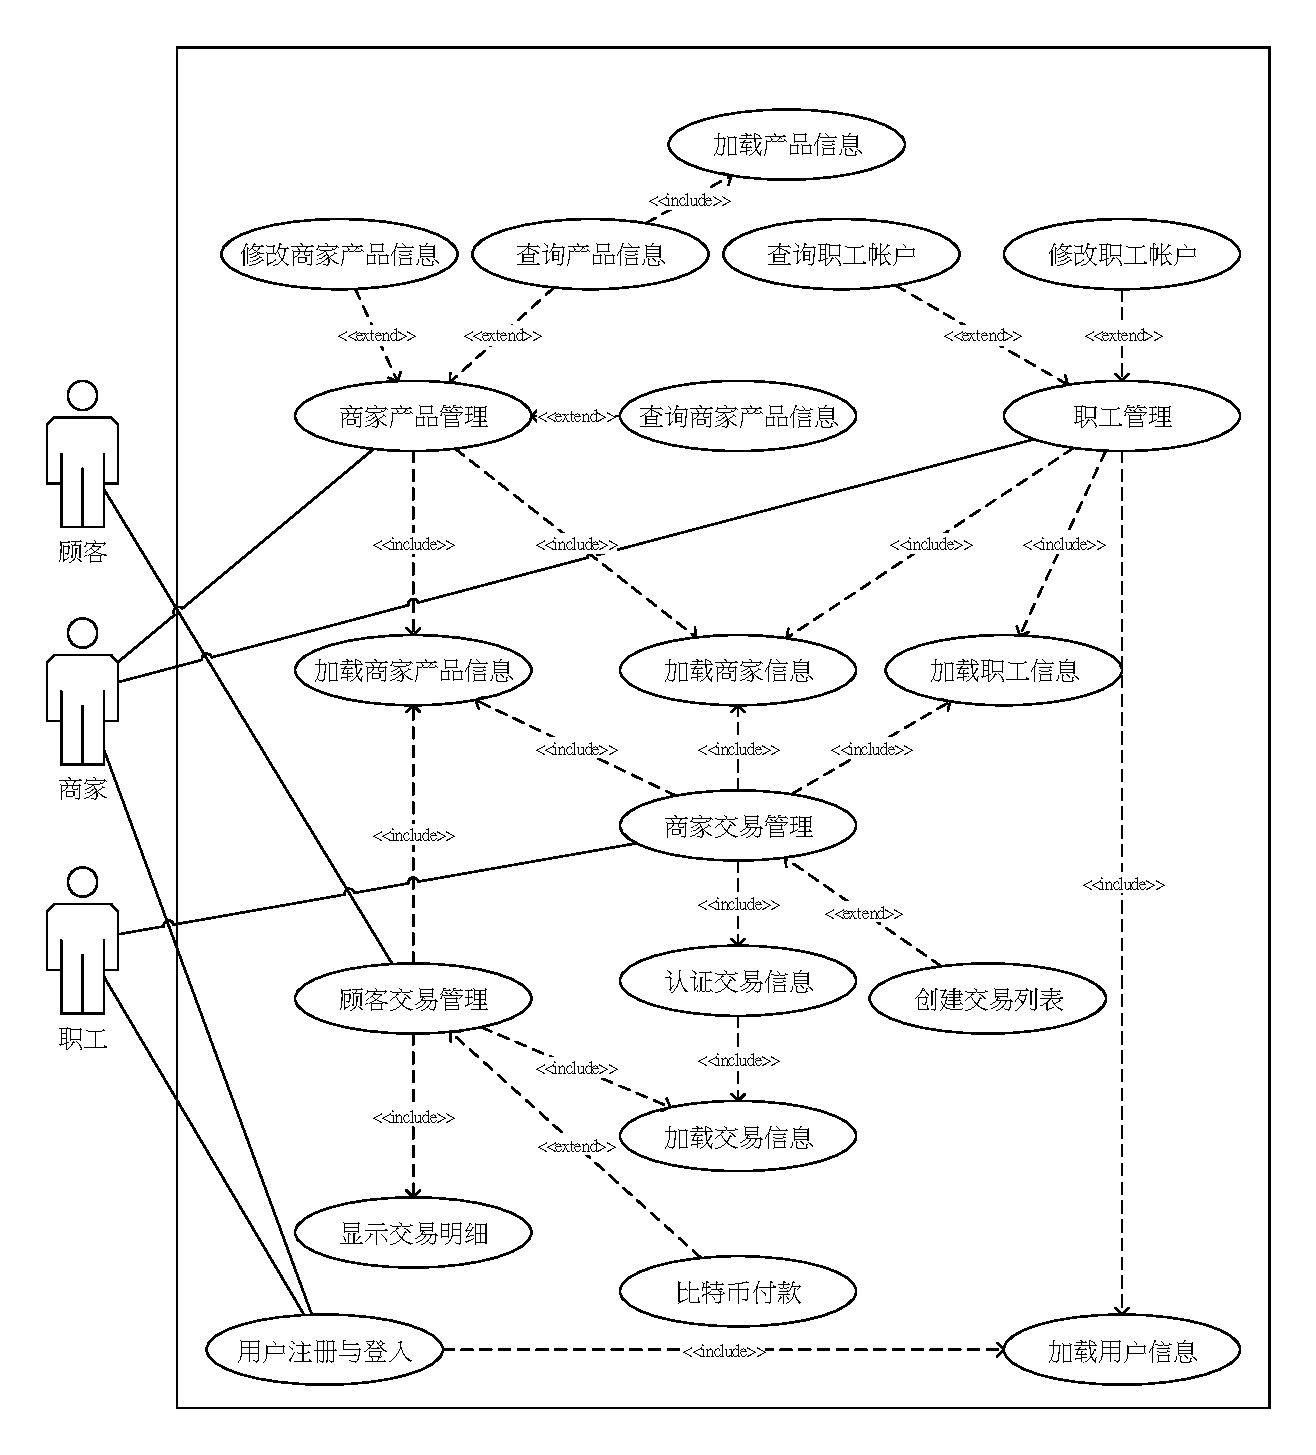
\includegraphics[width = 0.95\textwidth]{UC.pdf}
	\caption{比特币交易监督系统⽤例图}\label{UC}
	\end{figure}

	\section{非功能性需求分析}

	\subsubsection{(一)性能需求}
	
	本文所实践之系统为比特币的交易监督系统,参与者商家需要使用到商家和商品信息管理子系统,在参与者商家操作该子系统时,系统在设置完成后,于存储的过程中应于三秒内完成。于商家和商品信息管理子系统,商家端手持移动装置收银与交易明细系统应达到于两秒内完成子系统与数据库之间的信息传递以及信息存储,倘若商家与顾客在完成交易后,却无法得到快速的系统响应,这使得参与者顾客与职工迟迟无法收到⽀付完成的回复,甚至导致商家的交易塞车影响用户的消费体验。

	\subsubsection{(二)可拓展性}

	本论文提出的系统为比特币的交易监督系统雏形,于系统设计中将优先考虑最必要功能并加以实现,包括商家和商品信息管理子系统、商家手持移动装置收款及交易子系统以及客户端手持移动装置支付和交易子系统,于上述三个子系统中皆可以进行数据库字段的添加,使得交易信息、商家信息、商品信息、商家产品信息、用户信息以及职工信息更加的完备且更符合实际上业务需求。在未来甚⾄可以加⼊更完整的税务信息,使政府在税务计算⽅⾯可以大幅降低⼈⼒资源成本且更快速地进⾏税务统计,而库存管理⽅⾯可以加⼊库存预测的服务。

	\subsubsection{(三)可操作性}
	在本系统中的三个⼦系统中,为了将商家端⾏动收银与交易明细系统,以及客户端⾏动⽀付与交易明细系统实现在手持移动装置Android 操作系统上,于介⾯设计⽅⾯应给予商家⽤⼾以及顾客⽤⼾⼈性化的操作交互设计,以及于代码撰写⽅⾯应更加简洁,使得⽤⼾在启动本⼿持移动端应⽤程序时可以在最短的时间内完成初始化程序加载。除了针对⽤⼾交互⽅⾯的优化,也需要添加各个功能项⽬的使⽤说明,以及⽤⼾操作问题反馈,给予使用本系统的手持移动装置在应⽤程序上能快速的修正以提升⽤⼾体验。商家端建置与管理商品信息⼦系统是以Java 编程语⾔实现,针对参与者商家操作进⾏设计,该⼦系统需简单明确的呈现商家信息、产品信息以及商家产品信息,使参与者商家可以快速地查看所有商品,并添加、修改以及删除相关产品信息,包括价格、库存以商家产品描述。

	\subsubsection{(四)软件与硬件环境需求}
	表\ref{eva}为本文提出系统的软件与硬件环境需求,商家交易客户端与顾客交易客户端是建置在Android手持移动装置的应用程序,本文提出的交易方式为比特币,因此导入bitcoinj\supercite{Bitcoinclients}对比特币钱包进行管理,该套件可以生成比特币地址、同步比特币区块链、透过AES加密算法保护比特币钱包以及发起比特币交易至比特币网络。针对数据库的控制数据传输选用JDBC\supercite{JDBCdatabaseaccesswithJava:atutorialandannotatedreference}实现数据库的添加、修改、删除以及查找的功能,商家交易客户端与顾客交易客户端的手持移动装置必须要内置NFC监听器用来发送与接收交易信息。商家管理客⼾端是以Java 编程语⾔实现,软件环境中需⽀持Java ⼯作环境,服务器端则需要SQL 环境进行数据库搭建。


	\begin{table}[!htb]
	\centering
	\caption{环境需求表}
	\label{eva}
	\begin{tabular}{|c|c|c|c|}
	\hline
	- & 操作系统 & 软件 & 硬件 \\ \hline
	\begin{tabular}[c]{@{}c@{}}商家交易\\ 客户端\\ 与\\ 顾客交易\\ 客户端\end{tabular} & \begin{tabular}[c]{@{}c@{}}Android 4 \\ 或以上\end{tabular} & \begin{tabular}[c]{@{}c@{}}Java 7 或以上 \\ bitcoinj v0.14.6 \\ JDBC 4.2 或以上\\  Maven 3+\end{tabular} & \begin{tabular}[c]{@{}c@{}}存储容量:32 GB\\ 内存容量:2 GB\\ 网络需求:10 兆或以上\\ 传感器:NFC监听器\end{tabular} \\ \hline
	\begin{tabular}[c]{@{}c@{}}商家管理\\ 客户端\end{tabular} & \begin{tabular}[c]{@{}c@{}}Windows 7 \\ 或以上\end{tabular} & \begin{tabular}[c]{@{}c@{}}Java 7 或以上 \\ JDBC\end{tabular} & \begin{tabular}[c]{@{}c@{}}硬盘容量:100 GB\\ 内存容量:4 GB\\ 处理器:Core 2 Duo 或以上\\ 网络需求:10 兆或以上\end{tabular} \\ \hline
	服务器端 & \begin{tabular}[c]{@{}c@{}}Windows Server \\ 2003 \\ 或以上\end{tabular} & \begin{tabular}[c]{@{}c@{}}Microsoft SQL Server \\ bitcoin-qt 0.8.X 或以上 \\ Apache HTTP Server\end{tabular} & \begin{tabular}[c]{@{}c@{}}硬盘容量:1000 GB\\ 内存容量:16 GB\\ 处理器:Xeon E3 或以上\\ 网络需求:100 兆或以上\end{tabular} \\ \hline
	\end{tabular}
	\end{table}




%		\begin{figure}[!htb]
%			\centering
%			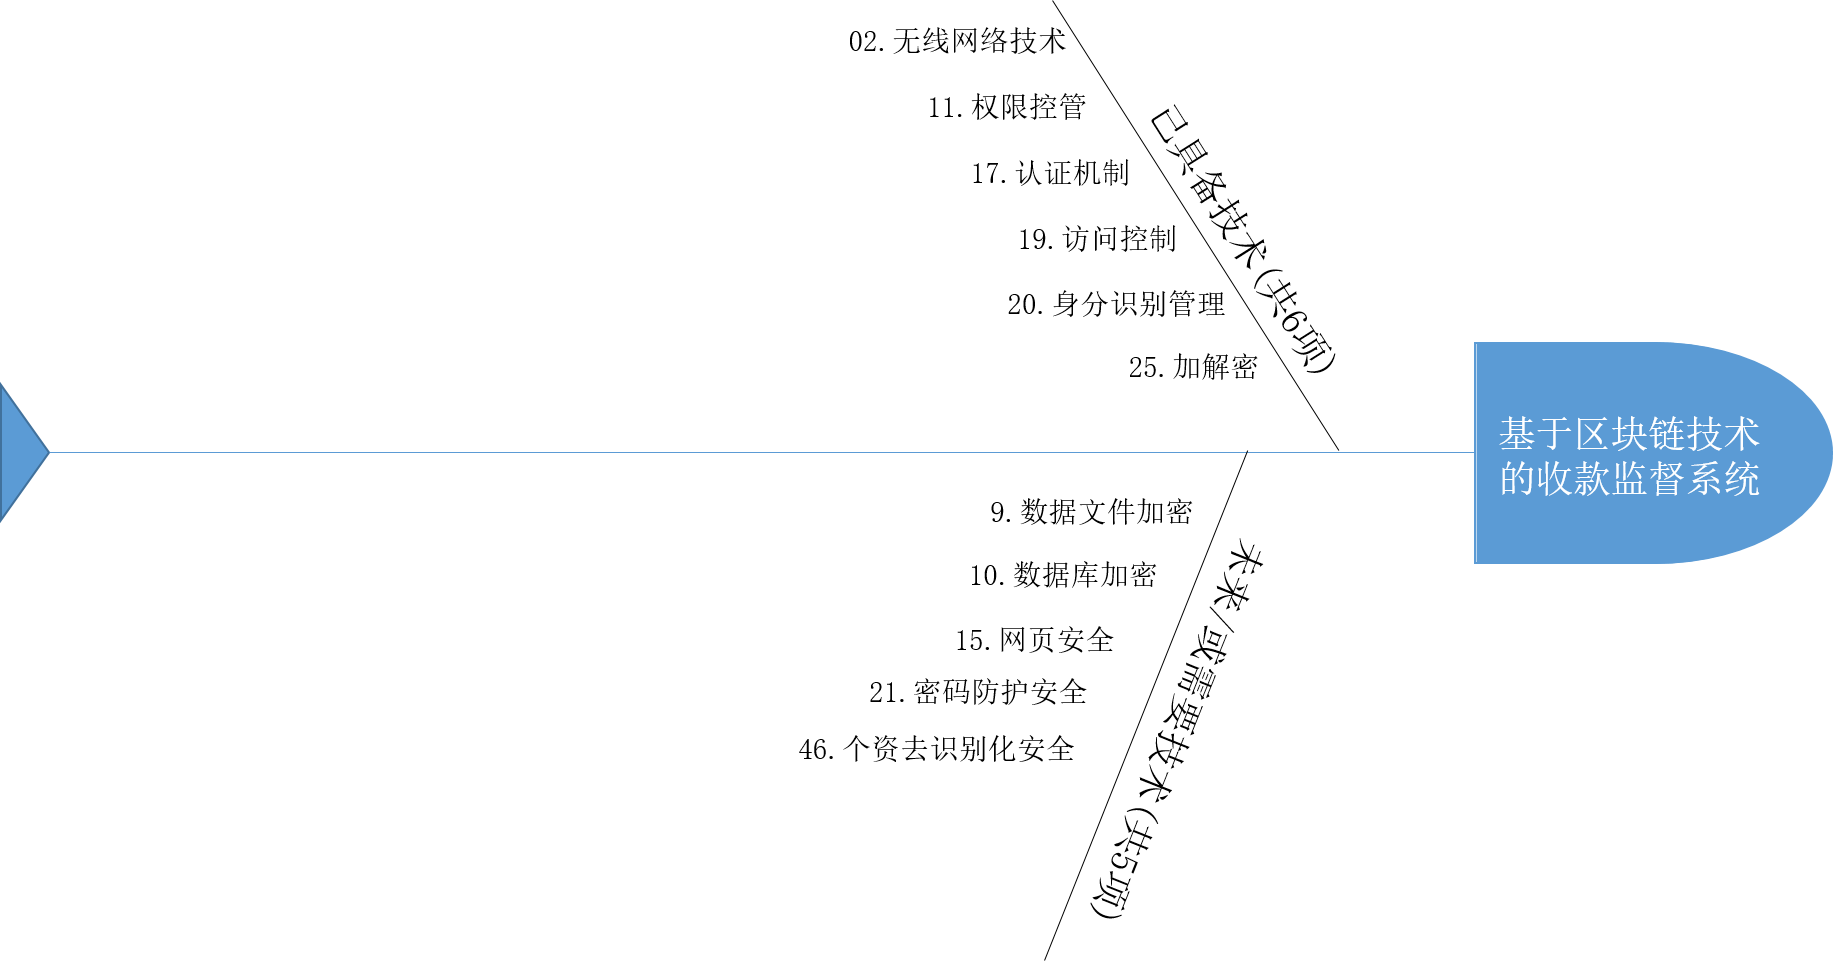
\includegraphics[width = 1\textwidth]{fish2.png}
%			\caption{鱼骨图(2)}\label{fish1}
%		\end{figure}

%		\subsection{匿名顾客对匿名商家}
%	\section{各种交易模型比较}
